\section{Partitioning}
\subsection{Models for System Synthesis}
\begin{itemize}
	\item Allocation + Binding = Partitioning
	\item Problem graph
\begin{itemize}
	\item Nodes: functional and communication task
	\item Edges: dependecies
\end{itemize}
	\item Architecture graph
\begin{itemize}
	\item Nodes: functional and communication resources
	\item Edges: directed communication resources 
\end{itemize}
	\item Specification graph
\begin{itemize}
	\item Problem graph + Architecture graph + Mapping edges
\end{itemize}
\end{itemize}

\begin{figure}
	\begin{center}
		\begin{subfigure}[b]{0.45\textwidth}
			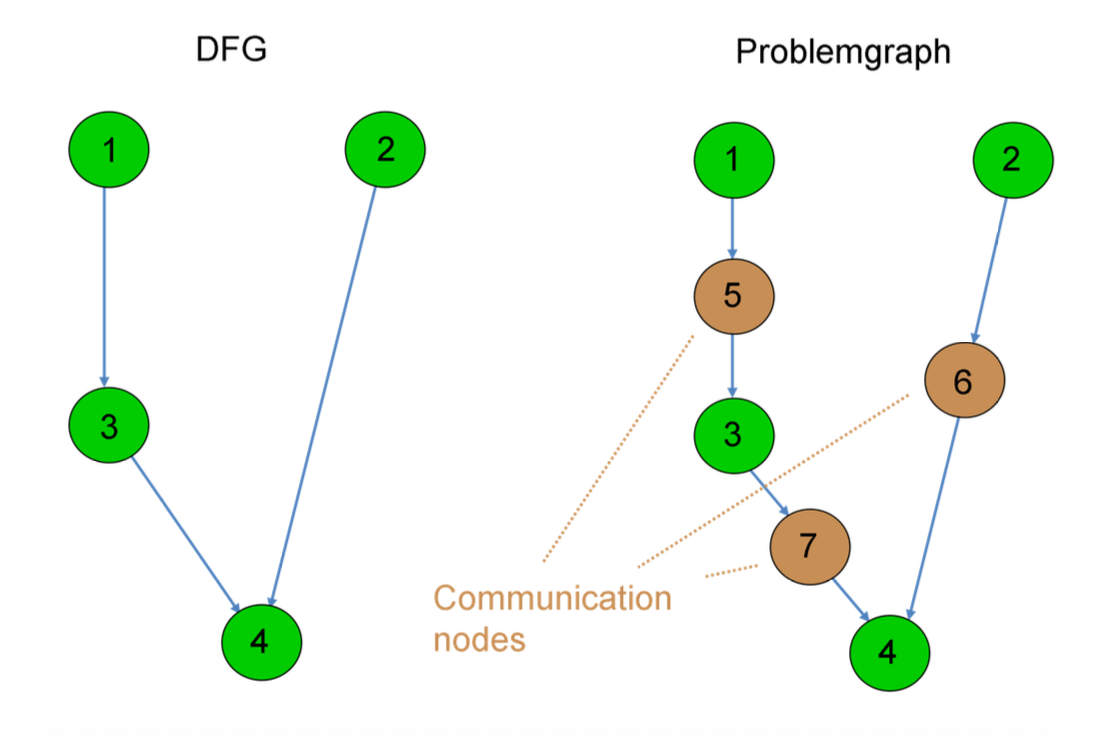
\includegraphics[width=\textwidth]{images/Problem_graph.png}
			\caption{Problem graph}
		\end{subfigure}
		\hfill
		\begin{subfigure}[b]{0.45\textwidth}
			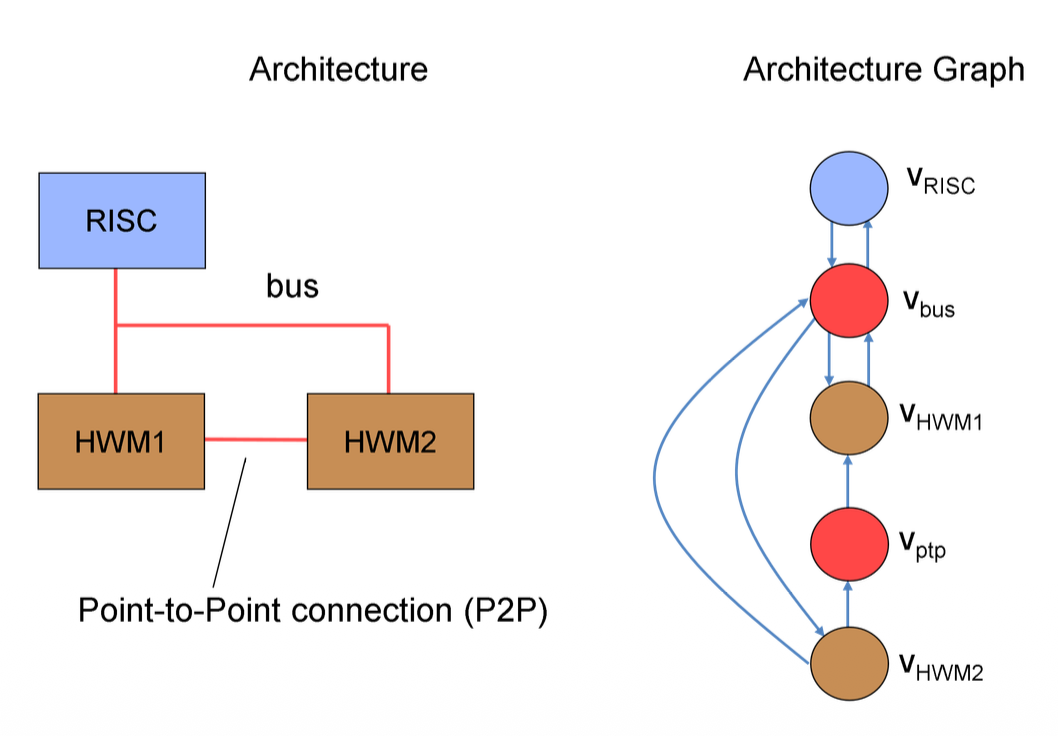
\includegraphics[width=\textwidth]{images/Architecture_graph.png}
			\caption{Architecture graph}
		\end{subfigure}
		\begin{subfigure}[b]{0.45\textwidth}
			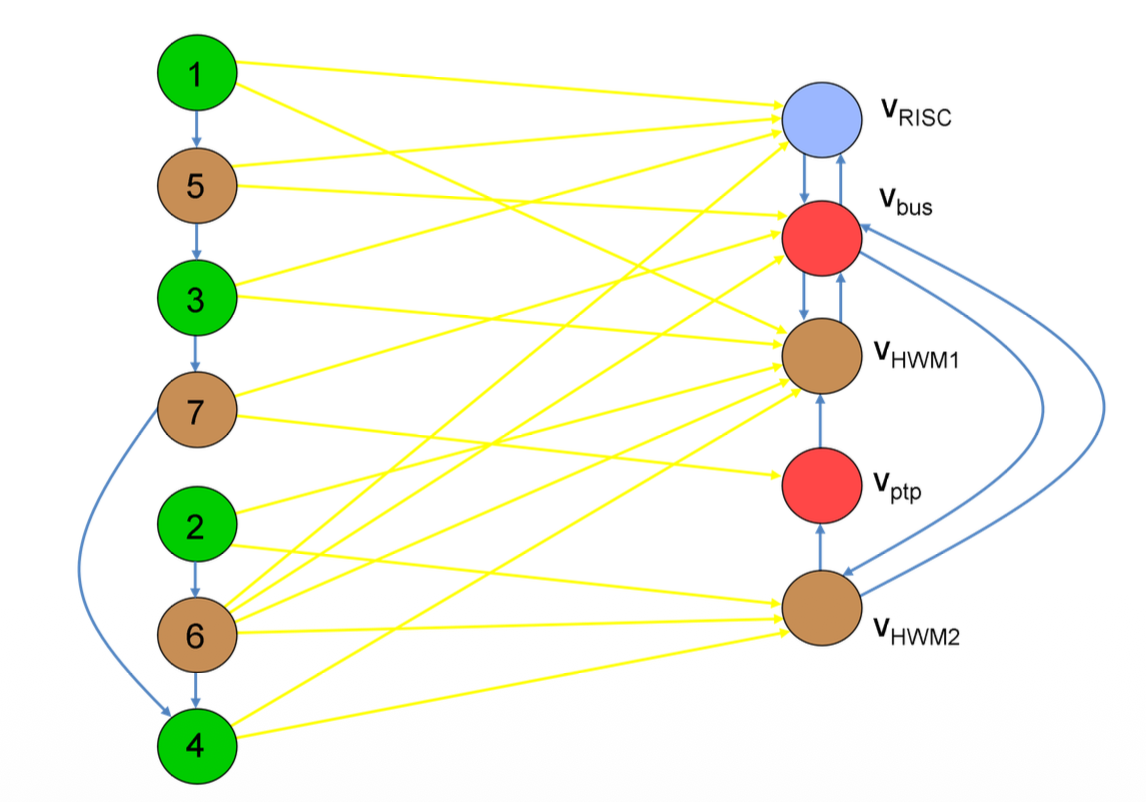
\includegraphics[width=\textwidth]{images/Specification_graph.png}
			\caption{Specification graph}
		\end{subfigure}
		\hfill
		\begin{subfigure}[b]{0.45\textwidth}
			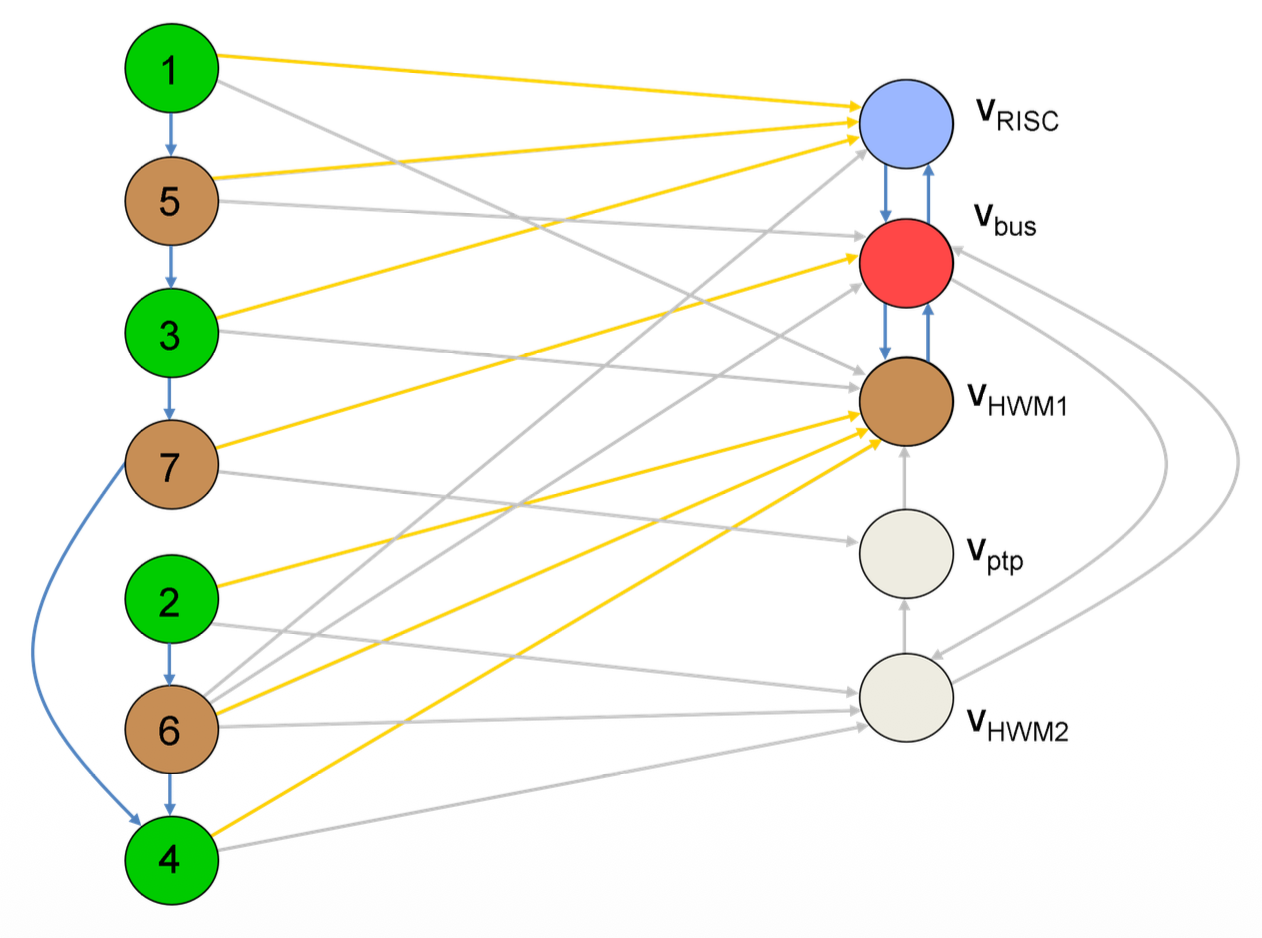
\includegraphics[width=\textwidth]{images/Allocation_binding.png}
			\caption{Allocation and binding}
		\end{subfigure}
		\caption{Models for System Synthesis}
		\label{fig:system_synthesis}
	\end{center}
\end{figure}

\subsection{Partitioning}
\begin{itemize}
	\item Abstraction level
\begin{itemize}
	\item Structural partitioning: RTL, netlists
\begin{itemize}
	\item System relatively well known
	\item No more comparison of design alternatives possible 
\end{itemize}
	\item Functional partitioning: system level
\begin{itemize}
	\item Comparison of design alternatives possible
	\item Quality of designs still not accurate
	$\rightarrow$ Estimation, Rapid Prototyping
\end{itemize}
\end{itemize}
	\item Cost( objective) function - Example:
\begin{itemize}
	\item $f(C, L, P) = k_1 \cdot h_c(C, \overline C) + k_2 \cdot h_L (L, \overline L) + k_3 \cdot h_p(P, \overline P)$
	\item System cost $C$, Latency $L$ and Power consumption $P$ 
\end{itemize}
	\item Problem definition: Group $n$ objects $O = \{o_1, \dots, o_n\}$ into $m$ blocks $P = \{p_1, \dots, p_m\}$ such that
\begin{itemize}
	\item $p_1 \cup \dots \cup p_m = O$
	\item $p_i \cap p_j = \emptyset \quad \forall i, j:i\not = j$
	\item while minimizing the cost $c(P)$
	\item The general partitioning problem is NP-complete
\end{itemize}
\end{itemize}

\subsubsection{General partitioning methods}
\begin{itemize}
	\item Heuristics
\begin{itemize}
	\item Constructive methods
\begin{itemize}
	\item Random mapping
	\item Hierarchical clustering (!!! Bullshit !!!)
\end{itemize}
	\item Iterative improvement methods
\begin{itemize}
	\item Kernighan-Lin algorithm
	\item Simulated Annealing
\end{itemize}
	\item Evolutionary algorithms
\end{itemize}
	\item Exact techniques
\begin{itemize}
	\item Enumeration of solution space
	\item Integer Linear Program (ILP)
\end{itemize}
\end{itemize}

\subsubsection{Constructive Methods}
\begin{itemize}
	\item Random Mapping
\begin{itemize}
	\item Each object is mapped randomly to a block
\end{itemize}
	\item Hierarchical clustering
\begin{itemize}
	\item Stepwise grouping of objects using a closeness function that indicates how beneficial it is to group two objects together
\end{itemize}
	\item Constructive methods
\begin{itemize}
	\item Are often used to fina an initial partition for methods of iterative improvement
	\item Have a problem in defining suitable closeness functions
\end{itemize}
\end{itemize}

\begin{figure}[h]
	\begin{center}
		\begin{subfigure}[b]{0.45\textwidth}
			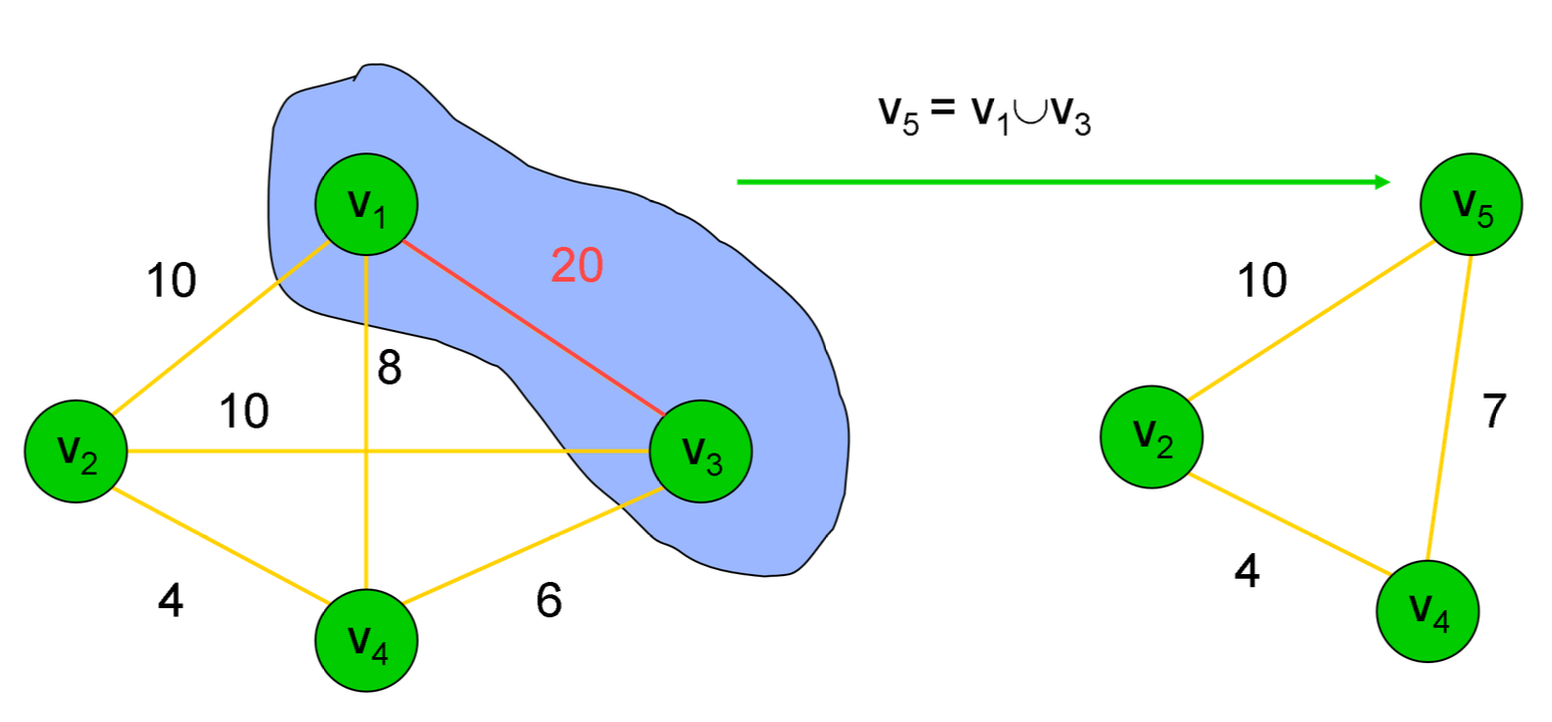
\includegraphics[width=\textwidth]{images/Hierarchical_clustering_1.png}	
		\end{subfigure}
		\hfill
		\begin{subfigure}[b]{0.45\textwidth}
			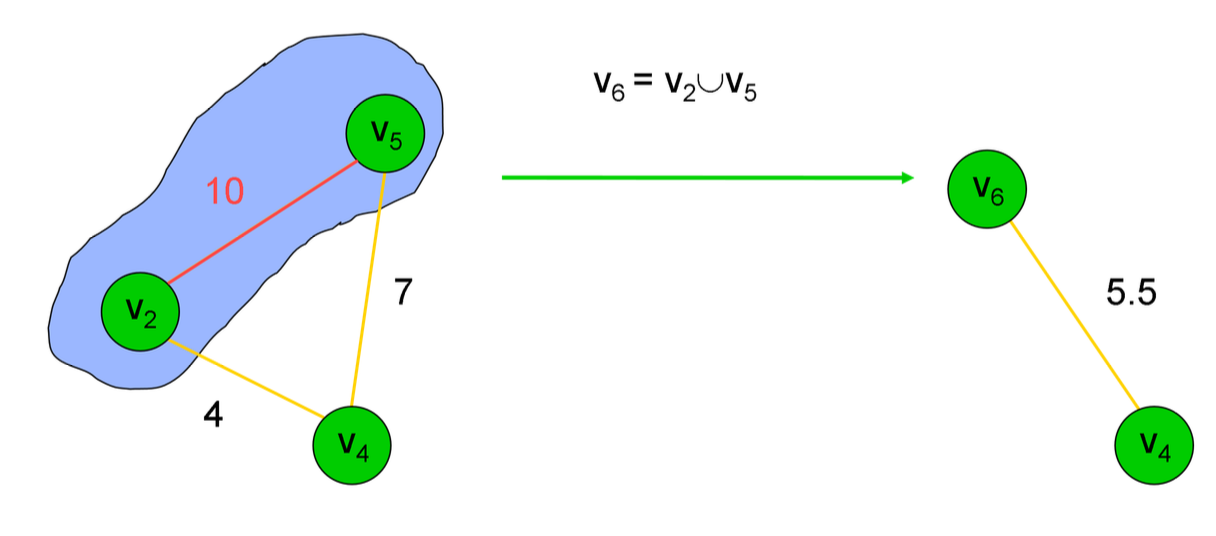
\includegraphics[width=\textwidth]{images/Hierarchical_clustering_2.png}	
		\end{subfigure}
		\begin{subfigure}[b]{0.45\textwidth}
			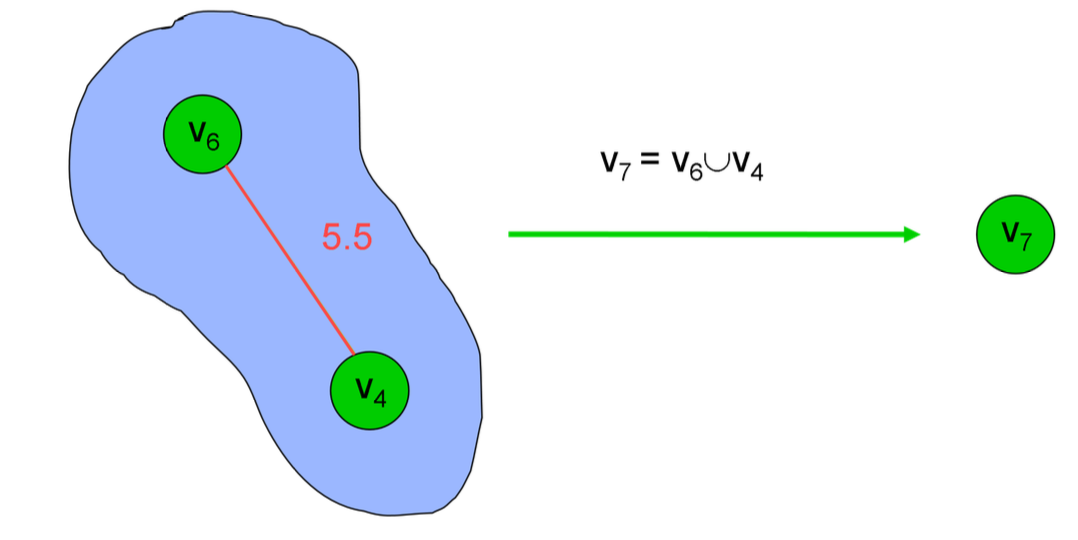
\includegraphics[width=\textwidth]{images/Hierarchical_clustering_3.png}	
		\end{subfigure}
		\hfill
		\begin{subfigure}[b]{0.45\textwidth}
			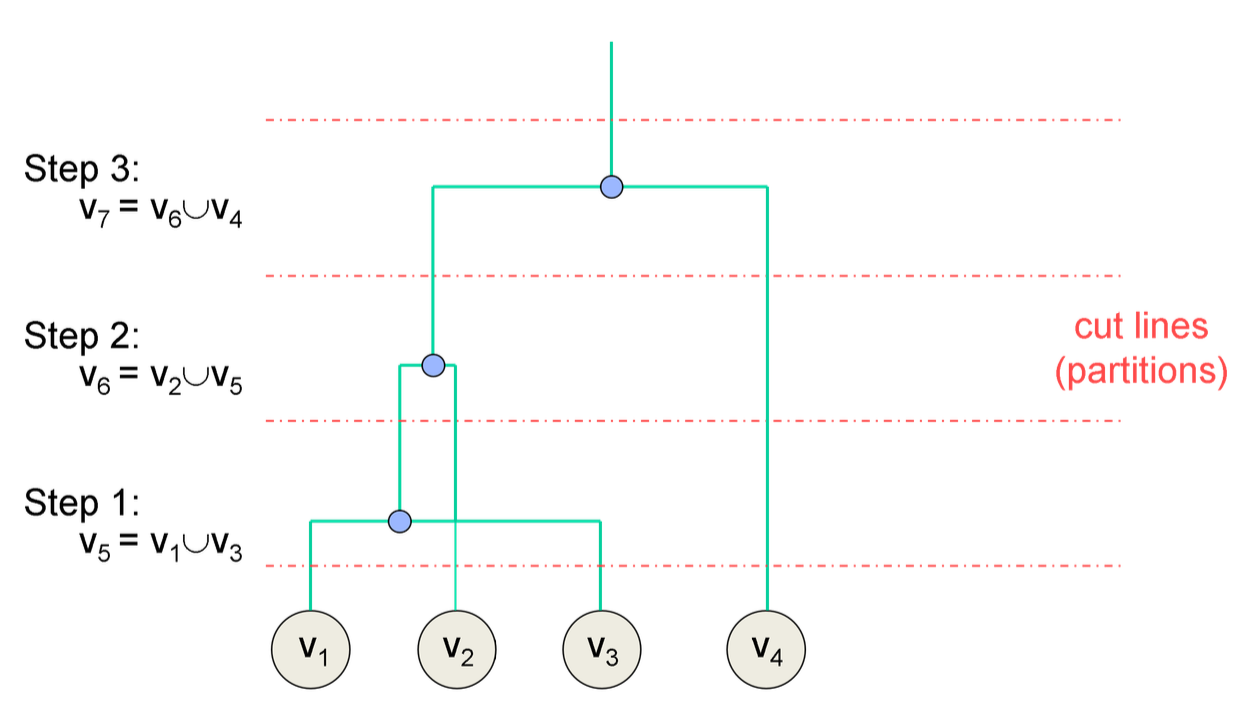
\includegraphics[width=\textwidth]{images/Hierarchical_clustering_4.png}	
		\end{subfigure}
	\end{center}
	\caption{Hierarchical Clustering - Example}
	\label{fig:hierarchical_clustering}
\end{figure}








